\documentclass[12pt]{report}
\usepackage[utf8]{inputenc}
\usepackage{amsmath}
\usepackage{amsfonts}
\usepackage{amssymb}
\author{Edward Seabrook} 
\title{Third Year Project Progress Report}

\usepackage[refpage]{nomencl}
\makenomenclature

% Makes Chapter heading look like Section heading
\usepackage{titlesec}
\titleformat{\chapter}% reformat chapter headings
    [hang]% like section, with number on same line
    {\Large\bfseries}% formatting applied to whole
    {\thechapter}% Chapter number
    {0.5em}% space between # and title
    {}% formatting applied just to title

% Save a bit of space by giving all headings less room
\titlespacing*{\chapter}{0pt}{0pt}{0pt}
\titlespacing*{\section}{0pt}{0pt}{5pt}
\titlespacing*{\subsection}{0pt}{0pt}{5pt}
\titlespacing*{\subsubsection}{0pt}{0pt}{5pt}
\titlespacing*{\paragraph}{0pt}{0pt}{5pt}

% Set margins to requied
\usepackage[top=2.4cm, bottom=2.4cm, left=3.5cm, right=2.4cm]{geometry} 

% Sort out margins for todonotes
\setlength{\marginparwidth}{3cm}
\reversemarginpar

% Set paragraph spacing to required
\setlength\parindent{0pt}
\usepackage[parfill]{parskip}

\usepackage{hyperref}
\usepackage{todonotes}
\usepackage{listings}
\usepackage{appendix}
\usepackage{pdflscape}


% Not totally sure
\usepackage{fancyhdr} 
\pagestyle{fancy} 
\renewcommand{\headrulewidth}{0pt} 
\lhead{}\chead{}\rhead{}
\lfoot{}\cfoot{\thepage}\rfoot{}

% Number and show in ToC to a deeper level
\setcounter{secnumdepth}{3}
\setcounter{tocdepth}{3}

\begin{document}

% Include title page

\begin{titlepage}

\begin{center}


% Upper part of the page
%\includegraphics[width=0.15\textwidth]{./logo}\\[1cm]    

\LARGE Electronics and Computer Science\\
Faculty of Physical and Applied Sciences\\
University of Southampton
\\[1.5cm]

\href{mailto:ejfs1g10@ecs.soton.ac.uk}{Edward JF Seabrook}\\[0.5cm]

\today \\[1cm]
{\bfseries A Tool to Simplify Network Administration in the Modern Home}\\[1.5cm]

\vfill

% Author and supervisor
\large
Project Supervisor: 
Dr.~T \textsc{Chown}\\

\large
Secondary Examiner:
Dr.~KP \textsc{Zauner} 

\vfill

A Project Progress Report Submitted for the Award of Computer Science

\end{center}

\end{titlepage}


\begin{abstract}
As home networks become more and more complex, it is inevitable that they will
require splitting into multiple subnets. As the average home user is unable to
configure a router, a minimal configuration solution is required. In this
project I set out to implement zero configuration OSPF based on a draft
published by the IETF. So far I have studied appropriate RFCs and selected a
base implementation. I have also set up the basic environment required for
continual testing.
\end{abstract}

\tableofcontents
\clearpage

\chapter{Project Description}
My initial project definition was very open ended as I was undecided between
two projects. I was unsure of both the scope of a third year project, and my
programming ability. The original project definition was to create
``a Tool to Simplify Network Administration in the Home''. The first potential
project was a home gateway monitor, the second was the project that
I have chosen. 

A more accurate title for my project is now ``Implementing Zero configuration
OSPFv3''. I shall be augmenting an existing implementation of the Open Shortest
Path First (OSPF) \nomenclature{OSPF}{Open Shortest Path First} network routing
protocol so that it doesn't require any configuration to effectively route
network traffic on a multiple subnet home network. The augmented implementation
will be tested to ensure that it works correctly both with homogeneous instances
and instances of alternative preexisting implementations. 

\section{Background}
As computing becomes more and more ubiquitous, the number of devices attached to
home networks will increase. It is difficult to predict all the possible uses of
network devices; some examples might include sensor networks to monitor the
home, network attached appliances such as ovens and dishwashers and surveillance
systems (e.g. CCTV). The Internet Engineering Task Force (IETF)
\nomenclature{IETF}{Internet Engineering Task Force} Home Networking (homenet)
\nomenclature{homenet}{Home Networking} working group is doing a lot of exciting
work into the evolution of networking in residential homes. 

With an increasing number of devices, network traffic will quickly become very
large. This is a problem that can be reduced by splitting the network into
multiple subnets. For example, a network for sensors, one for PCs and another
for appliances. 

Multiple subnets would also be a convenient way of enabling public access to a
home network. A subnet could be created for guests to connect to. This guest
network could provide some subset of the services of the main home network -
internet access could be provided but file sharing protocols such as Server
Message Block (SMB) \nomenclature{SMB}{Simple Message Block} would remain
unaccessible.

Routing is common place in large networks such as Universities or Businesses,
where full time network administrators set up and maintain the networks.
Unfortunately, most home users lack technical knowledge, instead they demand a
solution that can simply be plugged in and left alone. This is where my project
comes in. 

Another problem that this project takes into consideration is the gradual
transition from 32bit IPv4 \nomenclature{IPv4}{Internet Protocol Version 4} to
larger 128bit IPv6  \nomenclature{IPv6}{Internet Protocol Version 6} addresses.
As we run out of IPv4 addresses, ISPs \nomenclature{ISP}{Internet Service
Provider}  will be forced to start issuing IPv6 addresses to resolve the
problem.

\section{Goals}
There are a number of goals that the project aims to meet for it to be deemed
a success.

\subsection{Project Goals}
The following are things that the project should do:

\begin{itemize}
	\item Allow multiple subnets in the home; allow hosts to communicate
	from one subnet to another.
	\item Require no configuration: The user should not need to enter any 
	settings, they should simply plug in the router, and it should work.
	\item Produce something of value for the community. The code I produce  
	should adhere to style and quality guidelines to ensure it is useful.
	\item Verify past implementations of the drafts.
	\item Discover any ambiguities in the drafts.
\end{itemize}

\subsection{Personal Goals}
By the end of the project I would like to have:

\begin{itemize}
	\item A better understanding of the process of the creation of internet
	standards.
	\item The ability to implement network protocols. 
	\item Improved programming skills (Mainly C or C++).
	\item Learned about new tools and techniques.
\end{itemize}

\chapter{Background and Literature Research}
The reading that I have done for this project can be split into two categories:
Theoretical reading which covers the theory behind the protocols, and Practical 
reading covering the actual implementations to be used during the project.

\section{Theoretical Reading}
The majority of the information for this project is contained within various
Request For Comments (RFCs) and similar drafts. RFCs are memorandums published
by the IETF that are submitted for peer review. RFCs form the standards that are
used across the Internet. In this document, where a more recent RFC has
obsoleted an older RFC, I shall avoid mentioning the older document. 

\subsection{RFC 2328} 
This RFC defines the OSPFv2 routing protocol. The protocol is a current internet
standard. It gives a complete description of the data structures and algorithms
of OSPF for IPv4. The appendices of the document provides the reader with a
clear description of the packets that are used in OSPF for IPv4.

\subsection{RFC 5340}
This RFC defines the OSPFv3 protocol (OSPF for IPv6). The protocol is only a
proposed standard, but is very widely accepted.  Since OSPFv3 in general is
fairly similar to OSPFv2, the RFC describes only the differences between the two
protocols. 

\subsection{draft-dimitri-zospf-00}
This draft was published in 2002, and expired in 2003 - it never passed version
00.  However, it lays out many of the main concepts for later drafts. A method
was proposed for running a cut down version of OSPFv3 for routing both IPv4 and
IPv6 traffic without requiring any manual configuration. 

\subsection{draft-ietf-ospf-ospfv3-autoconfig-00} 
This draft defines OSPFv3 Auto-Configuration, it is the main draft that will be
used for this project, it provides a set of modifications that can be made to
the OSPFv3 protocol to run (in a slightly restricted manner e.g. single area)
it in without needing any manual configuration. The draft discusses
configurations that should be restricted to defaults, methods of selecting
Router-IDs (RID) and ways of detecting duplicate RIDs. 

The draft references many RFCs, a good understanding of the concepts 
that they convey is required to implement the draft successfully:

\begin{itemize}
	\item RFC 5838 - OSPFv3-AF (Address Families)
	\item RFC 6506 - OSPFv3-AUTH-TRAILER
	\item RFC 3630 (4230 \& 5786) - Traffic Engineering Extensions 
	\item RFC 4862 - iStateless address autoconfiguration (SLAAC for IPv6) 
\end{itemize}

\subsection{draft-arkko-homenet-prefix-assignment-03}
This draft is by the same author as the previous draft, it defines
Prefix Assignment in Home Networks. As a testament to how recent this work is, a
new version of this draft has been released since the beginning of this project. 

The memo describes a method for dividing an IPv6 prefix across the subnets of a
home network using Type Length Values (TLVs) in OSPF Link State Advertisements
(LSAs).

\subsection{Cisco's Guide to Configuring OSPFv3}
Aimed at network administrators, this document provides a nice high level
overview of the OSPFv3 Protocol. I found it useful to use this document to
understand the high level concepts without having to worry about low level
details.

\subsection{OSPF: Anatomy of an Internet Routing Protocol}
This book was written by the creator of OSPF, J. Moy. It defines the design and
structure of OSPF in a greater level of detail than the RFC.

\subsection{OSPF: Complete Implementation}
The companion of the first book, also written by J. Moy. Provides a complete
implementation and walks you through how it has been put together. This book and
it's companion were written before OSPFv3.

\subsection{OSPF and IS-IS}
Talks about choosing an IGP (Interior Gateway Protocol) for large networks,
giving a feature by feature comparison of OSPF with IS-IS (another distance
vector routing protocol). This book is mostly about OSPFv2 but does touch on
OSPFv3 towards the end.

\section{Practical Reading}		
The practical information for this project is mainly from online tutorials and
documentation of software projects.  

\subsection{alix2d3 Installation Guide}
This guide offered a comprehensive list of steps that need to be taken to
install Ubuntu Linux on a PC Engines alix2d3.  The article is written in
German but using Google translate I was able to follow it as it is mainly a list
of shell commands.

The process begins with installing the compact flash card as a device on an
existing Ubuntu desktop PC. Next the card is partitioned using \texttt{fdisk},
the card is then formatted as ext2 (a Linux file system type) using
\texttt{mk2fs}. The card is then mounted in the file system, using
\texttt{mount} and a small installation of Linux is copied to the card using
\texttt{debootstrap} to provide a base system.  

Several settings and devices are linked to the flash cards mount point and
\texttt{chroot} is used to simulate booting into the new install. The required
configuration files are edited (e.g. network interface settings) and essential
software packages (such as \texttt{Vim}, \texttt{SSH}, \texttt{sudo}, and
\texttt{APT}) are installed. A boot loader such as \texttt{GRUB} is also
installed and configured. 

Next, the flash card is safely removed, and  inserted into the alix2d3. The
alix2d3 is then powered on. Using a USB to Null Model cable connecting a PC to
the alix2d3's serial port, a terminal connection can be established using {\bf
cu}. I had a few problems using this device (\texttt{ttyUSB0}) but I was able to
fix this problem using \texttt{chown}. This terminal connection can be used to
aid the boot process and ensure that there are no Magic ELF errors. Once the
alix2d3 is up and running it is possible to disconnect the serial cable and
access it over \texttt{SSH} alone. 

\subsection{OSPF Implementations}
There are many different implementations of the OSPF protocol, the three most
popular open source implementations are XORP, Quagga and BIRD. Each of the
projects are well documented, they all use Git for version control and all have
active mailing lists (both user and developer).

\subsubsection{XORP}
XORP is Implemented in C++ following an Object Oriented style. OSPFv2 and OSPFv3
share much of the same code with conditional code separating the parts which are
different.

XORP implements OSPFv2 to comply with RFC2328 and OSPFv3 to the specification
defined in draft-ietf-ospf-ospfv3-update-23 (A draft version of RFC 5340).

\subsubsection{Quagga}
Quagga is a fork of the now defunct GNU Zebra project. It also implements
OSPFv3, taking a modular approach, providing an completely separate from OSPFv2.
The protocols are implemented in C using a mainly \texttt{struct} based style.
Vyatta, a software based virtual router, notably switched from XORP to Quagga. 

Quagga supports OSPFv2 as RFC 2328 and OSPFv3 to RFC2740. There are a few
differences between RFC2740 and RFC5240, these are listed in the latter.

\subsubsection{BIRD}
BIRD is a more lightweight implementation. It also makes use of C
\texttt{struct}s. It has been used before to successfully implement zero config
OSPF. 

BIRD complies to RFC2328 and RFC5240 in it's implementations of OSPF. 

\chapter{Design of System}
The design of my project has been done by individuals and groups of
people who have far more knowledge and experience working with networks than I
do. It is my job to understand these complicated designs and implement them
correctly.

\section{Chosen System}
I have chosen to base my project on Quagga for many reasons. Firstly, Quagga has
by far the most active mailing list. Secondly, Quagga splits up OSPFv2 and
OSPFv3 - they do not share any of the same source code; since I am only
concerned with OSPFv3, this should reduce the complexity involved with the
implementation. Quagga is also used by the Vyatta project, giving it a large
amount of exposure. 

I also found it easiest to install set up and use Quagga. It has a precompiled
package in Ubuntu's \texttt{APT} (Advanced Packaging Tool) repositories. One
reason I decided against using BIRD is that an implementation for a new platform
is more useful to the community. One potential downside to using Quagga is that
it uses plain \texttt{struct} based C, and I have more experience writing object
oriented code. 

\begin{figure}
\centering
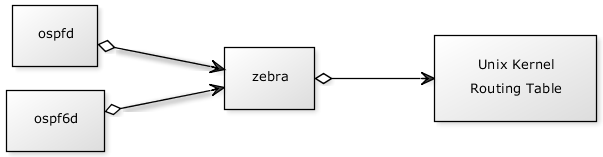
\includegraphics[width=\textwidth]{../Diagrams/UML/quaggaZebra.png}
\caption{Diagram of how Quagga is structured.}
\end{figure}

Quagga is split up into several daemons. A daemon is a program that is run as
a background process rather than interactively. Each of the daemons is
responsible for one protocol. \texttt{ospfd} runs the OSPFv2 protocol, and
\texttt{ospf6d} runs the OSPFv3 protocol. Each of these daemons makes use of 
\texttt{zebrad} to alter the systems routing table. 

As previously mentioned, Quagga is written in C and makes heavy use of
\texttt{struct}s to mimic object oriented programming, there is a
\texttt{struct} for each of the data structures defined in the RFC. 

\section{Test Networks}
To ensure the implementation works as expected, I will need to test instances of it
running on a few typical test networks. Figures \ref{fig:SimpleTestNet} and
\ref{fig:ComplexTestNet} show examples of possible test network.

\begin{figure}
\centering
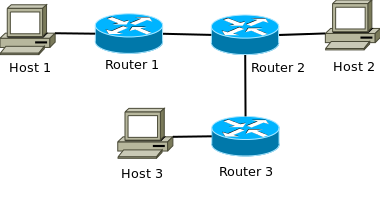
\includegraphics[width=0.75\textwidth]{../Diagrams/Network/SimpleTestNet.png}
\caption{Diagram of a simple test network. Typical in a future home network.}
\label{fig:SimpleTestNet}
\end{figure}

\begin{figure}
\centering
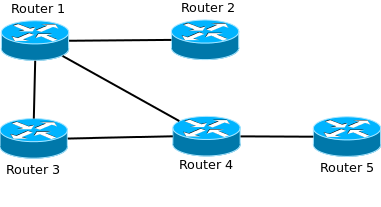
\includegraphics[width=0.75\textwidth]{../Diagrams/Network/ComplexTestNet.png}
\caption{Diagram of a more complex test network. Test more advanced features
such as multiple paths. Each router/link has implicit hosts.}
\label{fig:ComplexTestNet}
\end{figure}

\chapter{Report on Technical Progress}
So far, I have made good progress, I am well on my way to successfully
completing the project by the final deadlines.

\section{alix2d3}
The alix2d3s have been set up to run Ubuntu Linux, a description of the
approach can be found above. In the future it may be necessary to create a more
customised build for these devices, if for example I find performance to be
poor. So far they seem to have remained stable, both devices have an uptime of
over 28 days.

Quagga has been compiled and installed on one of the routers, and XORP on the
other. I installed BIRD to my desktop PC. I found compilation of the projects on
the alix2d3s to be very slow, in the future I shall use a more powerful
machine, for example a desktop PC.

\section{Reading}
All of the material mentioned above has been read lightly. As many of the
documents reference the other documents, I found them difficult to fully
understand, anything I am not confident about will be revisited once I have
a more solid foundation.

I have studied RFC 2328 (OSPFv2) and RFC 5340 (OSPFv3) in great depth making
detailed notes of their contents. I have also begun studying the appropriate
drafts.

As well as reading these documents, I have also looked at the source code of the
various implementation. After choosing Quagga, I began studying it's source code
in more depth to get an understanding of what changes need to be made. 

\section{Network Topologies}
I have also been thinking about network topologies that could be
used as test environments. These topologies need to test both typical home
networks, and stranger configurations that could result from inexperienced
people setting up the networks. 
 
As well as this I have begun attempting to assemble the networks that I have
suggested as test environments to ensure that I have sufficient hardware. 

\section{Progress Report}
Finally, I have written this document which has helped me formalise how my
project is coming along. Creating a Gantt chart, and other tasks, have helped me
to understand what I need to do to stay on track.

\chapter{Plan of Remaining Work}
My project will continue throughout the Christmas vacation although I have
decided to plan as though I shall not be working over Christmas (or Easter) to
ensure that I do have enough time to complete my project. The following tasks
still need to be completed.

\section{Study Quagga}
I will need to study in depth the source code of Quagga so that I have a
good idea of what needs altering to implement the required changes. I will
produce Class diagrams and other UML (Unified Modelling Language) diagrams to 
summarise the architecture of the software. The process of producing these
diagrams should help ensure that I understand the code. 

\section{Implementation}
Next will come the main work of the project. I will need to perform the required
changes to augment the Protocol to conform with the drafts. This section will
take a large proportion of the project's time, so I aim to start this as early
as possible. I shall begin by implementing as little as is required to make it
work, and then extending this in several iterations until I have a complete
product.

\section{Testing}
All projects require testing to ensure that they work as expected.

\subsection{Homogeneous Testing}
To verify that I have produced something that works, I shall test my
implementation homogeneously. I shall test it on the test network with all of
the routers running my implementation.  

\subsection{Heterogeneous Testing}
Networking protocols should not be implementation specific. As such, it should
be possible for my implementation to work harmoniously with the existing
implementations. If they do not work together, this would indicate that there is
a problem with my implementation, the old implementation or there is an
ambiguity in the specification.

\subsection{User Testing}
As my project is intended to be used by home users, it might be useful to also
test on potential users. The target audience would be technically able people
who have no experience of configuring multi-subnet networks. This will 
require ethics approval, so may not be possible.

\section{Extensions}
This project is open to a huge number of possible extensions if I finish
early.

\subsection{Multiple Hop Service Discovery}
As my project would create the possibility to have multiple subnets, a possible
extension is to investigate, and implement, multiple hop service discovery.
Essentially service discovery packets could be forwarded by the routers or
passed around inside the LSAs to enable a device on one subnet to see a service
advertised on another.

\subsection{Source Based routing}
It would also be possible to investigate source based routing. In a typical home
there is only one connection to the internet (usually ADSL), in the future it
may become more common for users to require multiple connections, see Figure
\ref{fig:MultipleISP}.  This could cause problems with traffic that needs to
respond being sent to the wrong gateway. Source based routing is a way of
preventing this by inspecting the source of the packet as well as it's
destination.

\begin{figure}
\centering
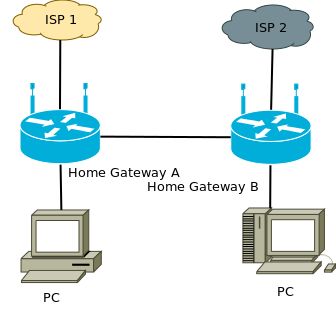
\includegraphics[width=0.75\textwidth]{../Diagrams/Network/MultipleISP.png}
\caption{Diagram of a network with multiple ISPs.}
\label{fig:MultipleISP}
\end{figure}

\chapter{Project Management}

\section{Tool and Techniques}
During the project I shall be making use of many tools and techniques.  One of
my goals is to learn about new tools,so I have tried to use tools that I only
have a small amount of experience working with. 

\subsection{Methodologies}
My project has a ridged specification so is not subject to change.
However, as the project is generally research based, I am uncertain of the scope
of the project. To combat this, I shall be using the spiral method. The project
shall be carried out in an iterative process of plan, implement and evaluate. I
also plan to use techniques from other methodologies such as Scrum. 

\subsection{Git}
I have chosen to use Git as my version control system. This choice was partially
because Quagga uses Git, however there are many other good reasons for using
Git, or any other Distributed Version Control System (DVCS). Firstly, version
control is essential to a software project as it enables you to keep track of
changes over time and revert to old versions if necessary. Distributed version
control is superior to traditional centralised version control system such as
subversion (SVN) as it allows work to be done without internet connectivity and
speeds up commit time (encouraging more frequent commits). I shall be
using bitbucket.org to back up my repository in the ``cloud''.

\subsection{Trello}
I shall be using Trello as a task management platform. Trello is a web app based
on Kanban. It provides card than can be placed into lists and moved around
between lists. Lists can have titles such as ``Thinking'', ``Doing'' and
``Done''. Trello will help me to keep track of tasks in my.

\subsection{Jenkins}
Jenkins is a continuous integration server, it can be configured to pull your
code from a repository and build it to ensure it still works.  

\subsection{\LaTeX}
I have chosen to produce all of the documentation associated with this project
using \LaTeX. I chose \LaTeX because it is a powerful tool that allows me to
focus on writing my report rather than typesetting. It also tends to be more
robust for longer documents than WYSIWYG editors such as Microsoft Word.

\subsubsection{Todonotes Package}
The package todonotes helps me keep track of ideas and tasks in my documents,
keeping my ideas separate from my finished work.

\subsubsection{Texcount}
As word counts are important throughout the project, I am using texcount to
count the words in my documents. Texcount parses the \LaTeX document so that
markup and headings are not counted.

\section{Risk Analysis}
Throughout my project there are many risks, I need to ensure that I take all the
possible precautions to limit the damage caused by these risks.

When using the power supplies, there is a risk that I could get an electric
shock. I took the power supplies to be PAT tested, as the power supplied are
double insulated (i.e. no single failure can result in a shock), a quick visual
inspection by a trained member of staff reassured me that they would be safe to
use. 

Around 01/12/2012, ECS had a fairly major network outage due to a hardware
failure. I was unable to do other coursework because I needed to use the
software within ECS. Making use of DVCS should help prevent this from being an
issue. I plan on replicating code and resources in ECS, at home and in the
cloud. 

Fire or some other unforeseeable event could damage to my data, in 2005 the old
Mountbatten building burned to the ground. To ensure that, if something like
this happens, I will not be affected, I shall make frequent backups of my work.

As my project involves using specialist hardware, there is a possibility that
the hardware could break. Fortunately the operating system (Ubuntu) that is
running on the alix2d3s is completely compatible with any x86 based computer. By
adding a second Network Interface Card (NIC) to my desktop PC, I am able to run
the software on there. 

I could have misjudged the difficulty of the project and be unable to complete
the project on schedule.  Because of this I have chosen to structure my project
in an iterative way, with different stages that I can attempt if I have time.
This approach should work quite well as my project is fairly research based. 

\pagebreak

\begin{landscape}

\section{Gantt Chart}
This Gantt chart shows how I have spent my time so far, and how I expect the
work to continued after the Christmas vacation.
\end{landscape}

\pagebreak

\printnomenclature

\pagebreak


\begin{thebibliography}{9}

\addcontentsline{toc}{chapter}{Bibliography}

\bibitem{heartImg}
	Flickr Image of Heart \\
	gustty,\\
	\url{http://www.flickr.com/photos/gustty/126606794/}


\end{thebibliography}

\begin{landscape}
\appendix 
%\appendixpage

\chapter{Typical Home Networks}
\section{Present}
\begin{center}
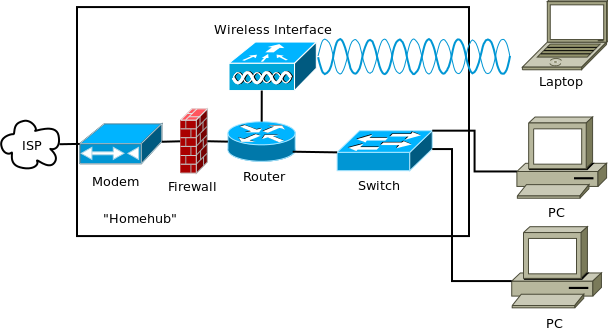
\includegraphics[width=0.75\linewidth]{../Diagrams/Network/TypicalHomenet.png}
\end{center}
This diagram shows a typical home network in the present day. The hardware
inside the box labeled ``Homehub'' is typically provided to customers as one
plug in and play device. It is commonly referred to as a router, although this
is slightly misleading as they perform many other tasks that routing.  

As can be seen from the diagram, the box provides the house with wired and
wireless connections to the LAN and the internet. The WLAN is typically bridged
with the LAN to give create a single subnet. 

\section{Future}
\begin{center}
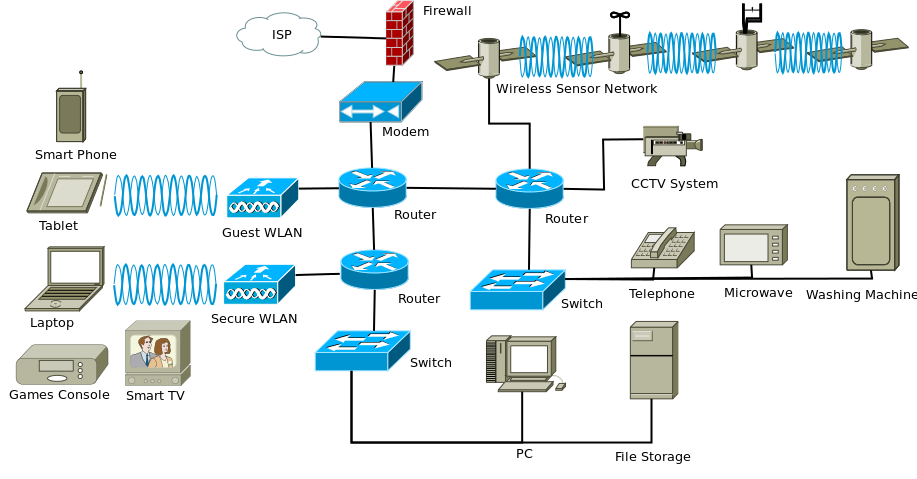
\includegraphics[width=0.9\linewidth]{../Diagrams/Network/FutureHomenet.png}
\end{center}
This diagram shows a hypothetical future home network. The network includes a
guest wireless network, a secured wireless network, a wired network, a network
for appliances, a network for a home surveillance system and a wireless sensor
network. 

\end{landscape}
\end{document}

